\section{Hardware-Based Dropping Architecture}
\label{sec:monitoring_hard_drop.hwdrop}

In Section~\ref{sec:monitoring_hard_drop.drop}, we presented a general
framework for how to design a system that allows dropping of monitoring tasks
to ensure the main task's execution time. However, implementing this framework
in software still has significant impacts on the WCET as shown in
Figure~\ref{fig:monitoring_hard_drop.drop.sw_drop_wcet}.  In this section, we
present a novel hardware architecture that eliminates these impacts to the main
task's WCET.

There are two main sources that affect the main task's WCET: the additional
code for keeping track of slack and the impact of the dropping task.  In
Section~\ref{sec:monitoring_hard_drop.hwdrop.slack}, we describe hardware to
keep track of slack and to make the decision on whether to run the monitoring
or dropping task.  In Section~\ref{sec:monitoring_hard_drop.hwdrop.drop}, we
present a hardware-based metadata invalidation scheme that allows dropping to
be performed in a single cycle.  By handling the dropping in a single cycle,
the throughput is able to match the throughput of the main core.
Section~\ref{sec:monitoring_hard_drop.hwdrop.filter} builds upon the
hardware-based invalidation scheme to filter out monitoring tasks for invalid
metadata in order to reserve slack for more useful cases of running the
monitoring task. Finally, in
Section~\ref{sec:monitoring_hard_drop.hwdrop.full_arch} we show the full
architecture.

\subsection{Slack Tracking}
\label{sec:monitoring_hard_drop.hwdrop.slack}

% Slack tracking hardware
\begin{figure}
  \begin{center}
    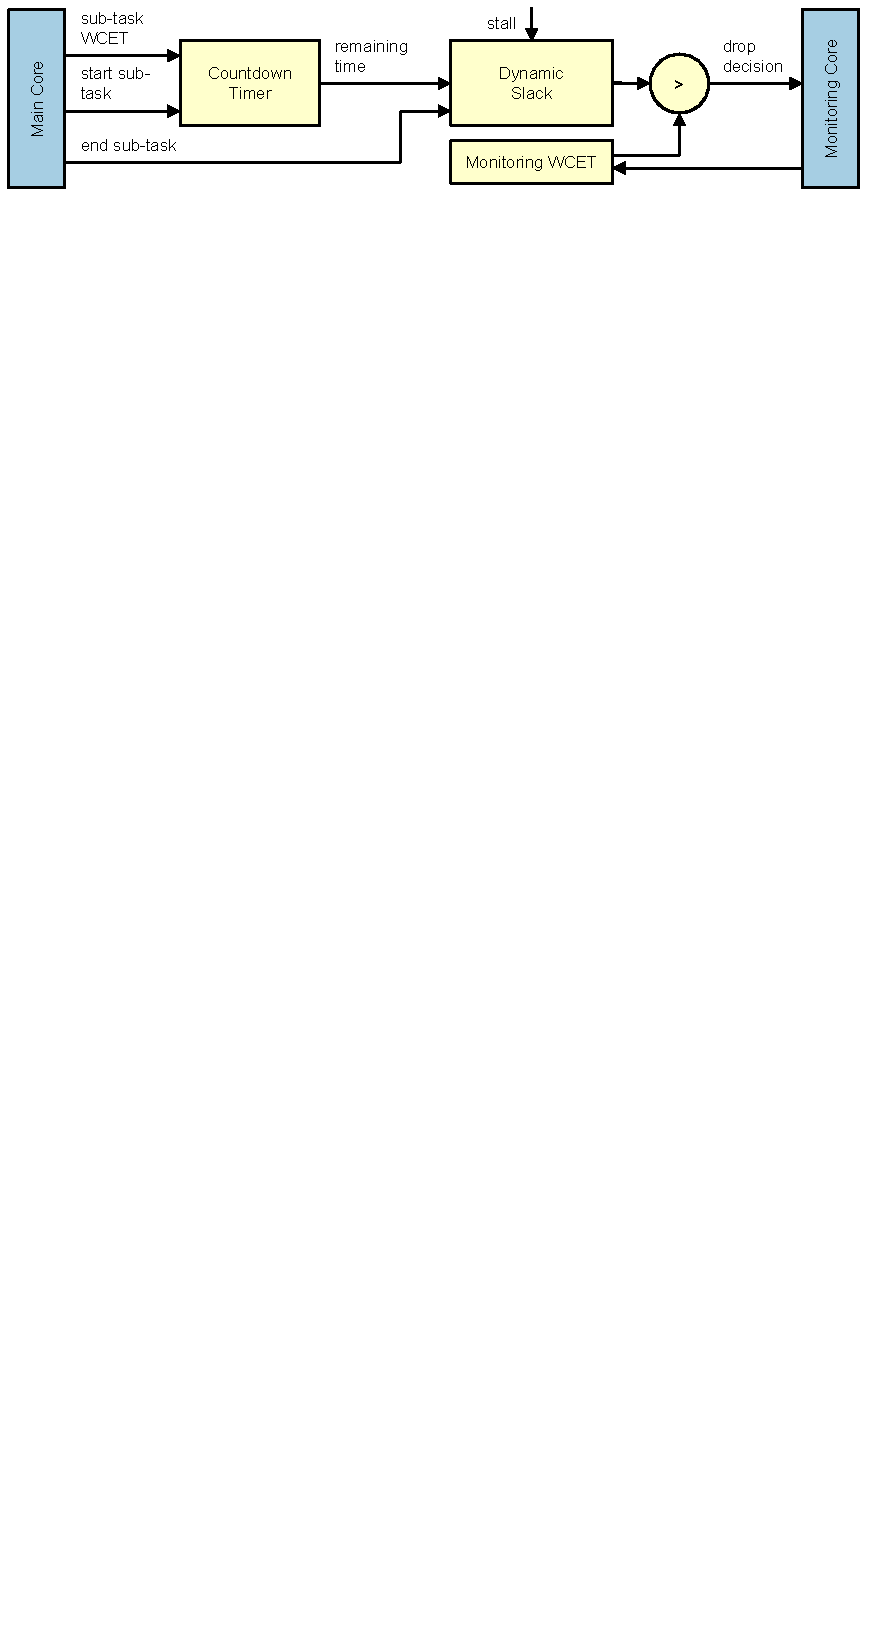
\includegraphics{monitoring_hard_drop/figs/slack_tracking.pdf}
    \caption{Hardware modules for keeping track of slack and making a drop decision.}
    \label{fig:monitoring_hard_drop.hwdrop.slack_tracking} 
  \end{center}
\end{figure}

Figure~\ref{fig:monitoring_hard_drop.hwdrop.slack_tracking} shows a hardware slack tracking module
(STM). In order to keep track of slack, a watchdog timer is loaded with a
sub-task's WCET at the start of a sub-task and counts down each cycle. At the
end of a sub-task, the remaining time in this watchdog timer is added to the
current dynamic slack which is stored in a register. At the start of a task,
the dynamic slack register is cleared and set to the headstart slack if one is
specified.  In addition, whenever the main task is stalled due to the
monitoring core, this dynamic slack is decremented.

The currently measured dynamic slack is used to determine whether the
monitoring task can run in full. When the monitor is initialized, the monitor
will load its worst-case needed slack in order to perform the monitoring task
into a register. When there is a monitoring event in the FIFO to be processed,
a hardware comparator checks whether the dynamic slack is greater than or equal
to the necessary slack for full monitoring. If enough slack exists, the
monitoring core is signaled to perform the monitoring task. Otherwise, the
monitoring event is dropped.

\subsection{Metadata Invalidation Module}
\label{sec:monitoring_hard_drop.hwdrop.drop}

% Metadata invalidation module
\begin{figure}
  \begin{center}
    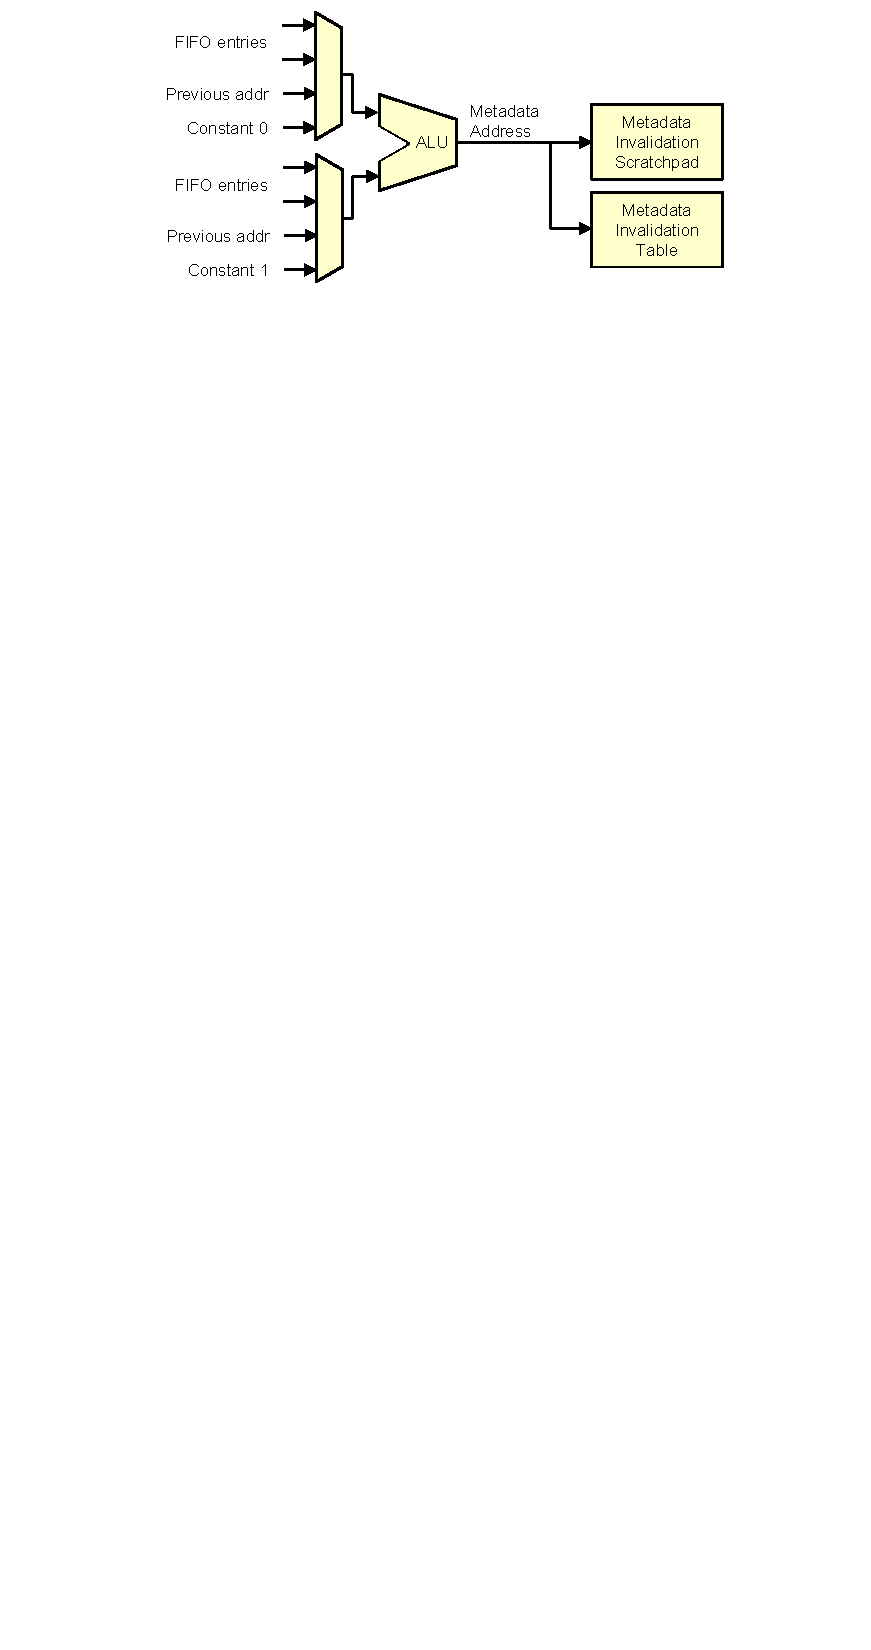
\includegraphics{monitoring_hard_drop/figs/mim.pdf}
    \caption{Metadata invalidation module (MIM).}
    \label{fig:monitoring_hard_drop.hwdrop.mim}
  \end{center}
\end{figure}

In the worst-case, all monitoring events must be dropped. Thus, it is important
that whatever dropping task needs to be run has a minimal impact on the main
task. If this dropping task can match the maximum throughput of the main core,
then the original WCET of the main task is not affected, removing the need to
redo the WCET analysis. In this section, we present a hardware architecture
that can handle dropping monitoring events in a single cycle, matching the
throughput of the main core.

As mentioned in Section~\ref{sec:monitoring_hard_drop.drop.dropping_tasks}, the dropping task must
invalidate metadata on a dropped monitoring event.  Thus, we have designed a
hardware module to perform this invalidation. Figure~\ref{fig:monitoring_hard_drop.hwdrop.mim} shows
a block diagram of this module, which we call the metadata invalidation module
(MIM).  When the slack tracking module indicates that a monitoring task must be
dropped, the metadata invalidation module sets a bit in the metadata
invalidation table (MIT) corresponding to the metadata to be invalidated.  The
metadata to be invalidated depends on the monitoring scheme and the monitoring
event. For example, for the uninitialized memory check monitoring scheme, on a
store event, metadata corresponding to the memory access address is set to
indicate initialized memory. Thus, on a dropped event, the MIM must be able to
calculate the address of this metadata in order to set a corresponding
invalidation flag.  The MIM includes a small ALU to perform these simple
address calculations. Since this metadata address mapping varies for different
monitoring schemes, the inputs to the ALU can either be data from the
monitoring event, the previous metadata address, or a constant. The input
selection and the ALU operation to perform are looked up from a configuration
table depending on the type of monitoring event.  The monitor sets up this
configuration table during initialization.

In order for this dropping operation to match the throughput of the main core
(i.e., up to one monitoring event per cycle), the metadata invalidation
information is stored on-chip. The MIT is implemented as a small on-chip
memory, similar to a cache. This memory stores invalidation flags and is
indexed using part of the metadata address. It stores the remaining portion of
the address as a tag. Unlike a cache, if an access misses in the MIT, there is
no lower-level memory structure to go to. This is done in order to ensure that
the MIM can handle a monitoring event every cycle. Instead of backing the MIT
with lower-level memory, if writing to the MIT would force an eviction, we
instead mark the corresponding cache set as ``aliased''. From this point on, we
are forced to conservatively consider any metadata that would be mapped to this
cache set as invalid, regardless of the tag corresponding to its metadata
invalidation address. This reduces the amount of useful monitoring that can be
done, but guarantees that the dropping hardware can match the main core's
throughput. These aliased sets can be reset by re-initializing (e.g., resetting
to a null value) all metadata that could map to the aliased set. By using
dynamic slack or a dedicated periodic task, the system can occasionally reset
aliased sets. In either case, a sufficiently sized MIT should ensure that
aliasing is rare.

In some cases we would like to use the MIM hardware to operate in such a way as
to ensure that aliasing does not occur. For example, we found that some
monitoring schemes save metadata information about registers. Since this
metadata is used often, it is important to manage it in such a way that
aliasing does not occur. Thus, the MIM also includes a metadata invalidation
scratchpad (MISP). This MISP is explicitly addressed and it is up to the system
designer to utilize it in such a way that aliasing will not occur.

Both the MIT and MISP are accessible by the monitor. This allows the monitor to
be aware of what has been invalidated. The monitor can also re-validate
metadata when possible, such as when the monitoring task writes metadata
values.

We note that the MIM was designed with the idea of marking certain metadata as
valid or invalid with a 1-bit flag. However, in general the MIM simply sets or
clears a bit based on a calculated address. We expect that for certain
monitoring schemes, designers may be able to use the MIM in new ways such as
using the MIT and MISP to directly express certain metadata.
Section~\ref{sec:extensions.dift} of the Appendix shows how the MISP can be
used to directly express the register file taint metadata used for a Dynamic
Information Flow Tracking (DIFT) scheme.

\subsection{Filtering Invalid Metadata}
\label{sec:monitoring_hard_drop.hwdrop.filter}

% Metadata filtering module
\begin{figure}
  \begin{center}
    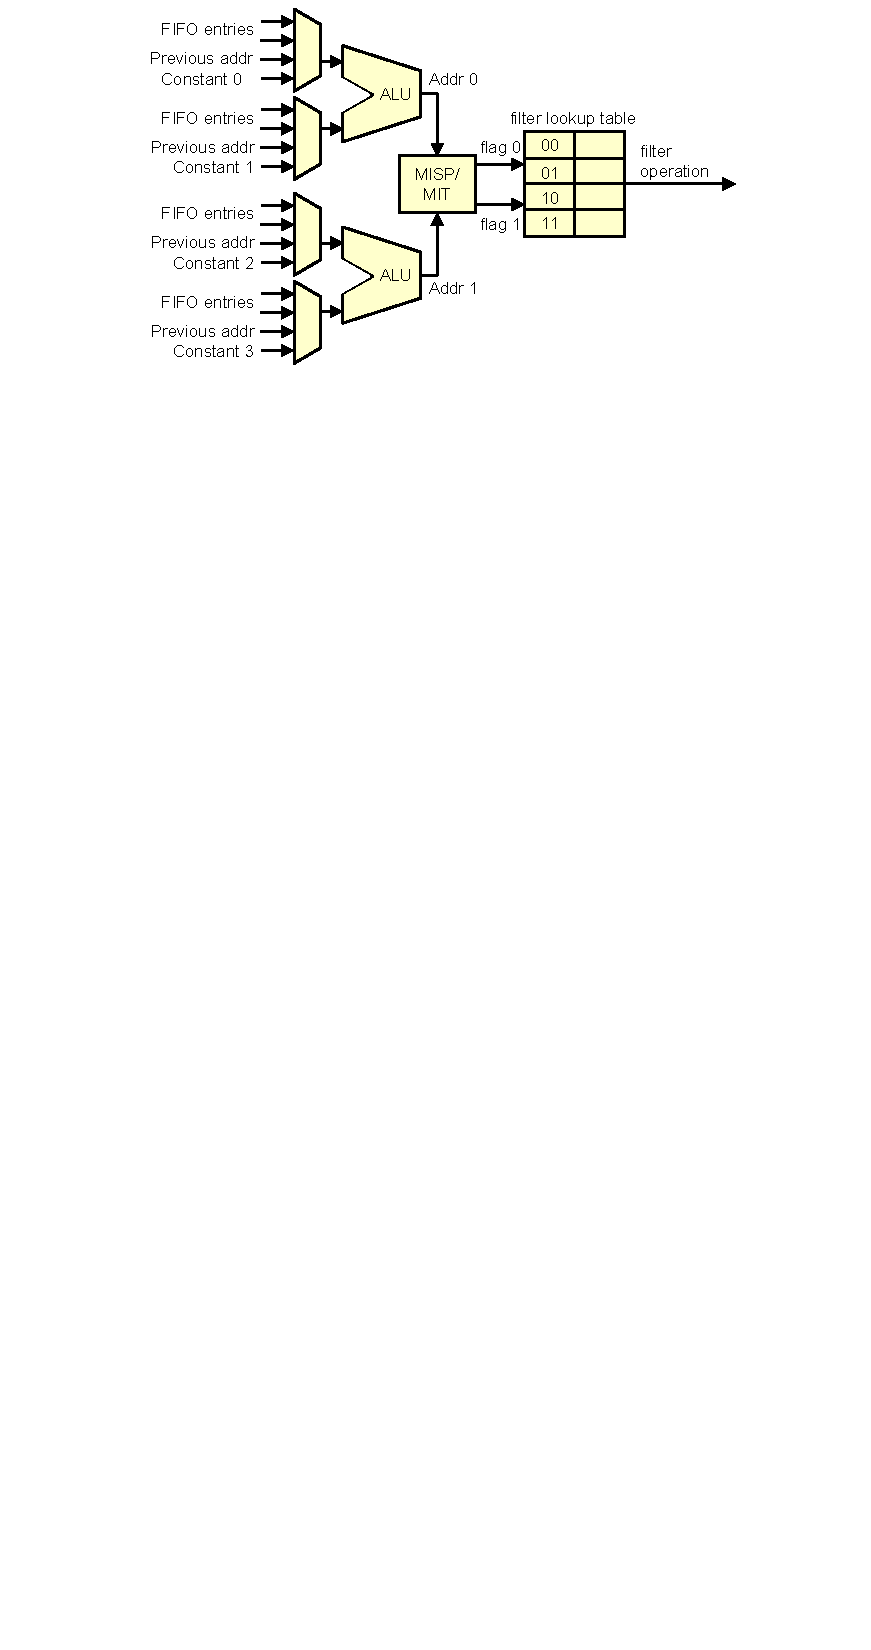
\includegraphics{monitoring_hard_drop/figs/mfm.pdf}
    \caption{Metadata filtering module (MFM).}
    \label{fig:monitoring_hard_drop.hwdrop.mfm}
  \end{center}
\end{figure}

Given that certain metadata becomes invalidated by the metadata invalidation
module, performing check and update monitoring operations based on the invalid
metadata is not useful. Thus, we can drop these monitoring tasks. By skipping
these invalid monitoring tasks, slack can be reserved for monitoring tasks
which operate on valid metadata. Determining when a monitoring event can be
filtered out in this manner is done by the metadata filtering module (MFM)
which is shown in Figure~\ref{fig:monitoring_hard_drop.hwdrop.mfm}.

We examined multiple monitoring schemes and found that most monitoring schemes
read in up to two metadata, corresponding to the two input operands of an
instruction, in order to perform an update.  Thus, the MFM was designed with a
pair of configurable metadata address generation units, similar to the ones
used in the MIM. These address generation units calculate a pair of addresses
which correspond to a pair of metadata invalidation flags which are read from
the MIT and/or MISP. The two flag bits are then used to look up an entry in a
lookup table that specifies whether to filter the event or not. Typically, if
either of the source metadata operands are marked as invalid, then the
monitoring task can be filtered. We must ensure no false positives occur due
to filtering out these monitoring events. Thus, the entry in the lookup table
can also inform the MIM of metadata that must be invalidated.  Similar to the
MIM, the monitor also configures the MFM address calculations and the lookup
table during initialization.

\subsection{Full Architecture}
\label{sec:monitoring_hard_drop.hwdrop.full_arch}

% Full hardware system
\begin{figure}
  \begin{center}
    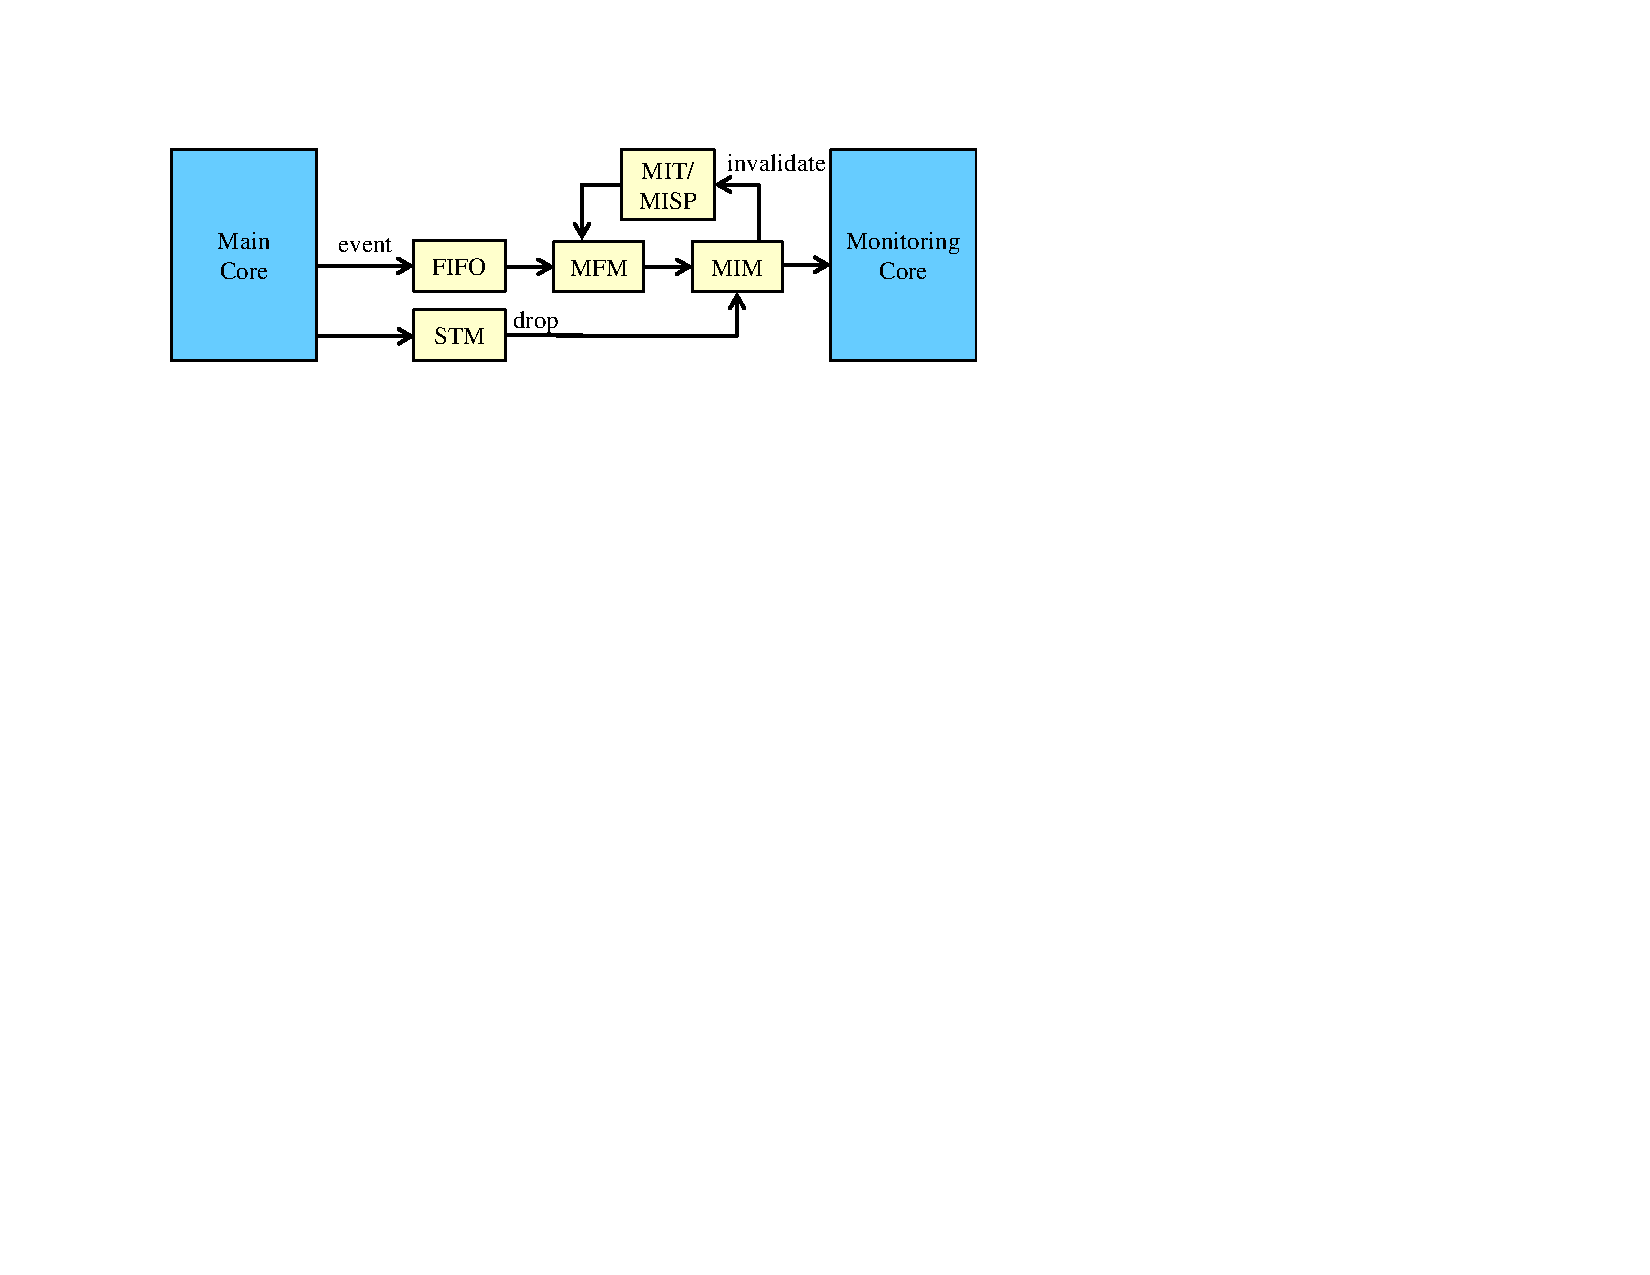
\includegraphics{monitoring_hard_drop/figs/full_hw.pdf}
    \caption{Block diagram of full hardware architecture for opportunistic
    monitoring on hard real-time systems.}
    \label{fig:monitoring_hard_drop.hwdrop.full_hw}
  \end{center}
\end{figure}

Figure~\ref{fig:monitoring_hard_drop.hwdrop.full_hw} shows a block diagram of the complete
architecture.  Monitoring events from the main core are first enqueued in a
FIFO. The events in the FIFO are dequeued and processed by the metadata
filtering module. The MFM checks the MIT and/or MISP to decide whether the
event should be filtered because of invalid metadata. If the event is not
filtered, then the metadata invalidation module decides whether to drop the
event based on the slack tracking module. If the event is dropped or filtered,
then the MIM marks invalidation flags using the MIT/MISP. Instead, if the event
is not dropped or filtered, then it is forwarded to the monitoring core to
perform the monitoring task.
